\documentclass{../template/texnote}

\title{\textbf{Learning is better than Programming}}[author={Linn Abraham}]

\begin{document}
    \maketitle \currentdoc{note}
    %<*note>
\section{Introduction}
The 2024 Nobel Prize in Physics was awarded to John J. Hopfield and Geoffrey E. Hinton for ``for foundational discoveries and inventions that enable machine learning with artificial neural networks''.
%In this article, we focus on Geoffrey Hinton and try to unravel the contributions he has made to the field.
The aim of this article is to understand a few concepts in the field by turning our attention to the contributions of Geoffrey Hinton.
Hinton is often called the ``The Godfather of A.I.'', whereas the title of ``Father of A.I.'' is often credited to either John McCarthy or Alan Turing.
What are his most significant contributions to the field?
%Let's pick three of his most important ones.
In the 1980s he showed that the backpropogation algorithm discovered by Rumelhart (and independently by others before him) could be used for learning representations from data.
In the work that was published in ``Letters to Nature'' he applied backpropogation to enable a machine learn the distributed representation of words.
However the hype that ensued fizzled down over the next twenty years or so years as researchers felt dissillusioned.
In 2012, he again showed the power of a deep Convolutional Neural Network (CNN) namely AlexNet by winning the ILSVRC challenge by a large margin.
Hinton was also the first to describe the Restricted Boltzmann Machines (RBM) which forms the basis of Deep Belief Networks (DBN).
In the rest of the article, let us try to understand how AlexNet changed computer vision and AI in general.

\section{ImageNet Challenge}
In a special edition of the original AlexNet paper, the authors give credit to the ImageNet dataset for the deep learning revolution.
The ImageNet dataset took about two years to be put together and was the basis of the ImageNet Large Scale Visual Recognition Challenge (ILSVRC) which began in 2010.
It is important to note that the ImageNet datastet is built upon the hierarchical structure provided by WordNet.
Each meaningful concept in WordNet was called a synonym set or `sysnet'.
WordNet has 80,000 such sysnets and the goal of ImageNet was to have approximately 500 to 1000 images per sysnet.
These sysnets are part of the many subtrees such as mammal, bird, fish, reptile, amphibian, vehicle, furniture, musical instrument, geological formation, tool, flower, fruit.
Figure \ref{fig:subtree} shows images from two of those subtrees.
    \begin{figure}
    \begin{center}
	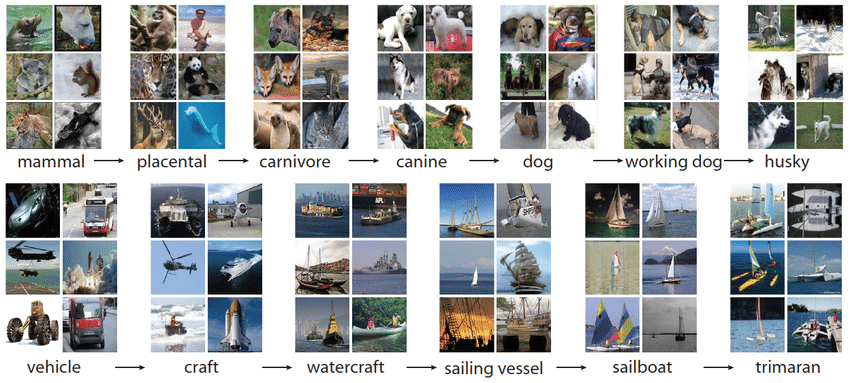
\includegraphics[width=\textwidth]{Linn/subtrees.png}
    \end{center}
    \caption{Image showing two of the subtrees and associated images in the ImageNet dataset.}
    \label{fig:subtree}
    \end{figure}
The year 2012 probably marked the the point when the ice began to melt after a long AI winter.
The winners of the first two years made use of intelligent features derived from images that researchers painstakingly came up with such as SIFT, Fisher vectors etc.
This they combined with shallow Machine Learning algorithms like Support Vector Machines (SVM), Principal Component Analysis (PCA) and others.
But in 2012 the team SuperVision consisting of Alex Krizhevsky, his Ph.D. supervisor Geoffrey E. Hinton and Ilya Sutskever put forward the AlexNet model.
It obliterated the competition, beating the runner up in top-5 error rates by more than 10 percentage points.
% define top-5 error
For each sample in the test set, each entry model provides a probability of being the right answer. A top-5 error only considers an error when the actual label 
is not amongst the top-5 most probable answers.
% challenge tasks?
	\begin{figure}
	\begin{center}
		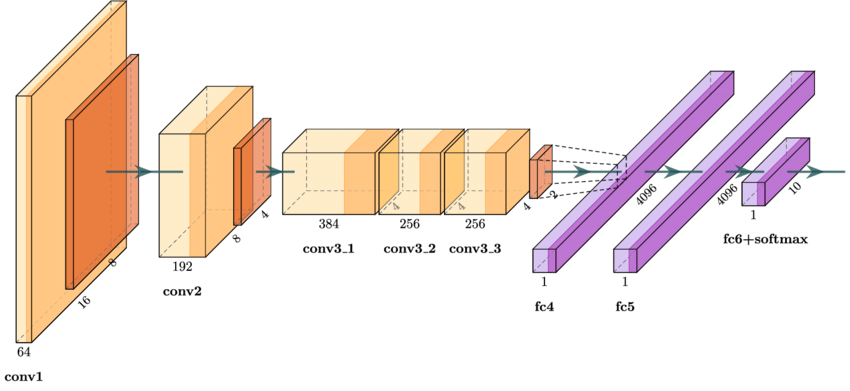
\includegraphics[width=\textwidth]{Linn/alexnet-architecture.png}
	\end{center}
	\caption{Diagram showing the architecture of the AlexNet model.}
	\label{fig:alexnet}
	\end{figure}
\section{AlexNet}
By winning the ILSVRC challenge with a huge margin, the authors proved without doubt that deeper networks were the answer.
%The novelty of their work was that they demonstrated for the first time the superiority of a deep Convolutional Neural Network (CNN) in image classification tasks.
%What is the AlexNet model?
%So let us try to understand what this model is about.
Before thinking about the implications of their discovery let us first try to understand what their model is all about.
The AlexNet model can be shortened as follows.

(CNN → RN → MP)² → (CNN³ → MP) → (FC → DO)² → Linear → softmax

It consists of eight layers, the first five being convolutional layers (CNN) and followed by three fully connected (FC) layers.
Figure \ref{fig:alexnet} shows a representative diagram of this architecture.
The CNNs had a ReLU activation which they found to be faster to train than tanh neurons.
They also implement local response normalization (RN) on the output of the CNN.
Some of the convolutional layers are followed by max-pooling layers (MP).
The final layers consists of a 1000 way softmax layer.
All in all, it had 60 million parameters and 650,000 neurons.
The network was trained on the large ImageNet dataset. Since the images from the dataset had arbitrary rectangular shapes, these were first downsampled to a resolution of 
$ 256 \times 256 $.
The authors also incorporated data augmentation by using image translation and horizontal reflections with patches of $227 \times 227$.
This increased their training set by a factor of 2048 although the generated images are highly correlated.
This means that during testing they would extract a similar patch from all four corners and a centre patch and pool the decisions of the network on all these five patches 
and their horizontal reflections.
%\section{Learning beats programming}
\section{The Legacy of AlexNet}
By 1986, partly due to the work of Hinton and others it was known that the Multi-Layer Perceptron was capable of learning any decision surface.
And the backpropogation algorithm was what made it possible to train networks with many layers.
However how would this fare when applied to tasks as complex as human vision?
For certain visual recognition tasks such as hand written digit recognition using the MNIST dataset it might be feasible to think of an MLP solution.
However in a much more general classification or detection task such as that put out by the ILSVRC, it became obvious that what was important was not just the pixel intensities in the images.
It was known that humans vision involved a hierarchy of features computed from the intensities like shapes, edges and textures.
Thus researchers came up with the convolutional neural network that would allow the machine to learn such features without exactly specifying what features where to be learnt.

    \begin{figure}
    \begin{center}
	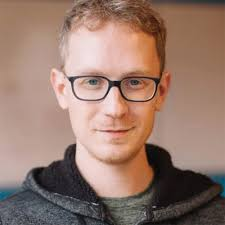
\includegraphics[width=0.4\textwidth]{Linn/alex.jpeg}
	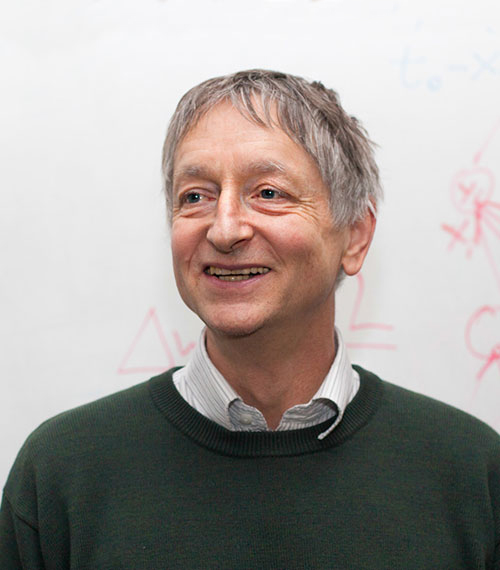
\includegraphics[scale=0.32]{Linn/hinton.jpg}
    \end{center}
    \caption{On the left, Alex Krizhevsky and on the right, Geoffrey Hinton.}
    \label{fig:}
    \end{figure}
    
The researchers behind AlexNet showed that less was more, by not hard coding intelligent features into their model but still allowing for the model to learn such features from data, 
They showed that learning was better than programming in solving such complex tasks.
They also showed that the depth of the network was critical to the result that they had achieved. They showed this by removing a convolutional block from their network and showing the 
performance degrade substantially.
Finally to practically train such deep networks they made use of the GPU by writing implementations of the 2D convolution operation and other associated operation which could make use of 
GPUs. They also made use of two GPUs by cleverly distributing the network between those.
Ever since GPUs have come to dominate the world of deep learning.
Dedicated frameworks like tensorflow, pytorch etc. were developed to make it easier than ever for deep learning researchers to make use of GPUs without getting their hands dirty.
In summary they showed that what was lacking was better and more data and more computation and not the algorithms.
%\end{document}
%\nocite{russakovskyImageNetLargeScale2015}
%\nocite{rosebrockDeepLearningComputer2017}
%\nocite{fordArchitectsIntelligenceTruth2018}
%\nocite{marslandMachineLearningAlgorithmic2014}
%\nocite{krizhevskyImageNetClassificationDeep2017}
%\nocite{dengImageNetLargescaleHierarchical2009}
\begin{thebibliography}{6}
\providecommand{\natexlab}[1]{#1}
\providecommand{\url}[1]{\texttt{#1}}
\expandafter\ifx\csname urlstyle\endcsname\relax
  \providecommand{\doi}[1]{doi: #1}\else
  \providecommand{\doi}{doi: \begingroup \urlstyle{rm}\Url}\fi

\bibitem[Russakovsky et~al.(2015)]{russakovskyImageNetLargeScale2015}
Olga Russakovsky, Jia Deng, Hao Su, Jonathan Krause, Sanjeev Satheesh, Sean Ma, Zhiheng Huang, Andrej Karpathy, Aditya Khosla, Michael Bernstein, Alexander~C. Berg, and Li~{Fei-Fei}.
\newblock {{ImageNet Large Scale Visual Recognition Challenge}}.
\newblock \emph{arXiv:1409.0575 [cs]}, January 2015.

\bibitem[ros(2017)]{rosebrockDeepLearningComputer2017}
\emph{Deep Learning for Computer Vision with {{Python}}: Practitioner Bundle}.
\newblock PyImageSearch, United States, 1st edition 1.3 edition, 2017.
\newblock ISBN 978-1-72248-783-6.

\bibitem[Ford(2018)]{fordArchitectsIntelligenceTruth2018}
Martin~R. Ford.
\newblock \emph{Architects of Intelligence: The Truth about {{AI}} from the People Building It}.
\newblock Packt Publishing, Birmingham, UK, 2018.
\newblock ISBN 978-1-78913-151-2.

\bibitem[Marsland(2014)]{marslandMachineLearningAlgorithmic2014}
Stephen Marsland.
\newblock \emph{Machine {{Learning}}: {{An Algorithmic Perspective}}}.
\newblock {Chapman and Hall/CRC}, 2 edition, October 2014.
\newblock ISBN 978-0-429-10250-9.
\newblock \doi{10.1201/b17476}.

\bibitem[Krizhevsky et~al.(2017)Krizhevsky, Sutskever, and Hinton]{krizhevskyImageNetClassificationDeep2017}
Alex Krizhevsky, Ilya Sutskever, and Geoffrey~E. Hinton.
\newblock {{ImageNet}} classification with deep convolutional neural networks.
\newblock \emph{Communications of the ACM}, 60\penalty0 (6):\penalty0 84--90, May 2017.
\newblock ISSN 0001-0782, 1557-7317.
\newblock \doi{10.1145/3065386}.

\bibitem[Deng et~al.(2009)Deng, Dong, Socher, Li, {Kai Li}, and {Li Fei-Fei}]{dengImageNetLargescaleHierarchical2009}
Jia Deng, Wei Dong, Richard Socher, Li-Jia Li, {Kai Li}, and {Li Fei-Fei}.
\newblock {{ImageNet}}: {{A}} large-scale hierarchical image database.
\newblock In \emph{2009 {{IEEE Conference}} on {{Computer Vision}} and {{Pattern Recognition}}}, pages 248--255, Miami, FL, June 2009. IEEE.
\newblock ISBN 978-1-4244-3992-8.
\newblock \doi{10.1109/CVPR.2009.5206848}.

\end{thebibliography}
    %</note>
    \printbibliography
\end{document}
